\section{Introduction}

Robot motion control can be implemented in two primary ways: open loop and feedback.

\subsection{Open loop control}
In open loop control, the mobile robot follows a predetermined trajectory computed beforehand, typically composed of motion segments from the starting point to the destination. 
The robot executes this planned trajectory without feedback until it reaches the goal.

The main challenges associated with open loop control include:
\begin{itemize}
    \item Difficulty in precomputing a feasible trajectory.
    \item Constraints and limitations on the robot's velocities and accelerations.
    \item Inability to handle dynamic changes such as obstacles.
    \item Lack of error recovery mechanisms.
\end{itemize}

\subsection{Feedback control}
In contrast, feedback control involves recomputing or adapting the trajectory online, utilizing a simple control scheme for path following. 
This approach adjusts the robot's orientation by modulating angular velocity and controls its distance by adjusting linear velocity.
\begin{figure}[H]
    \centering
    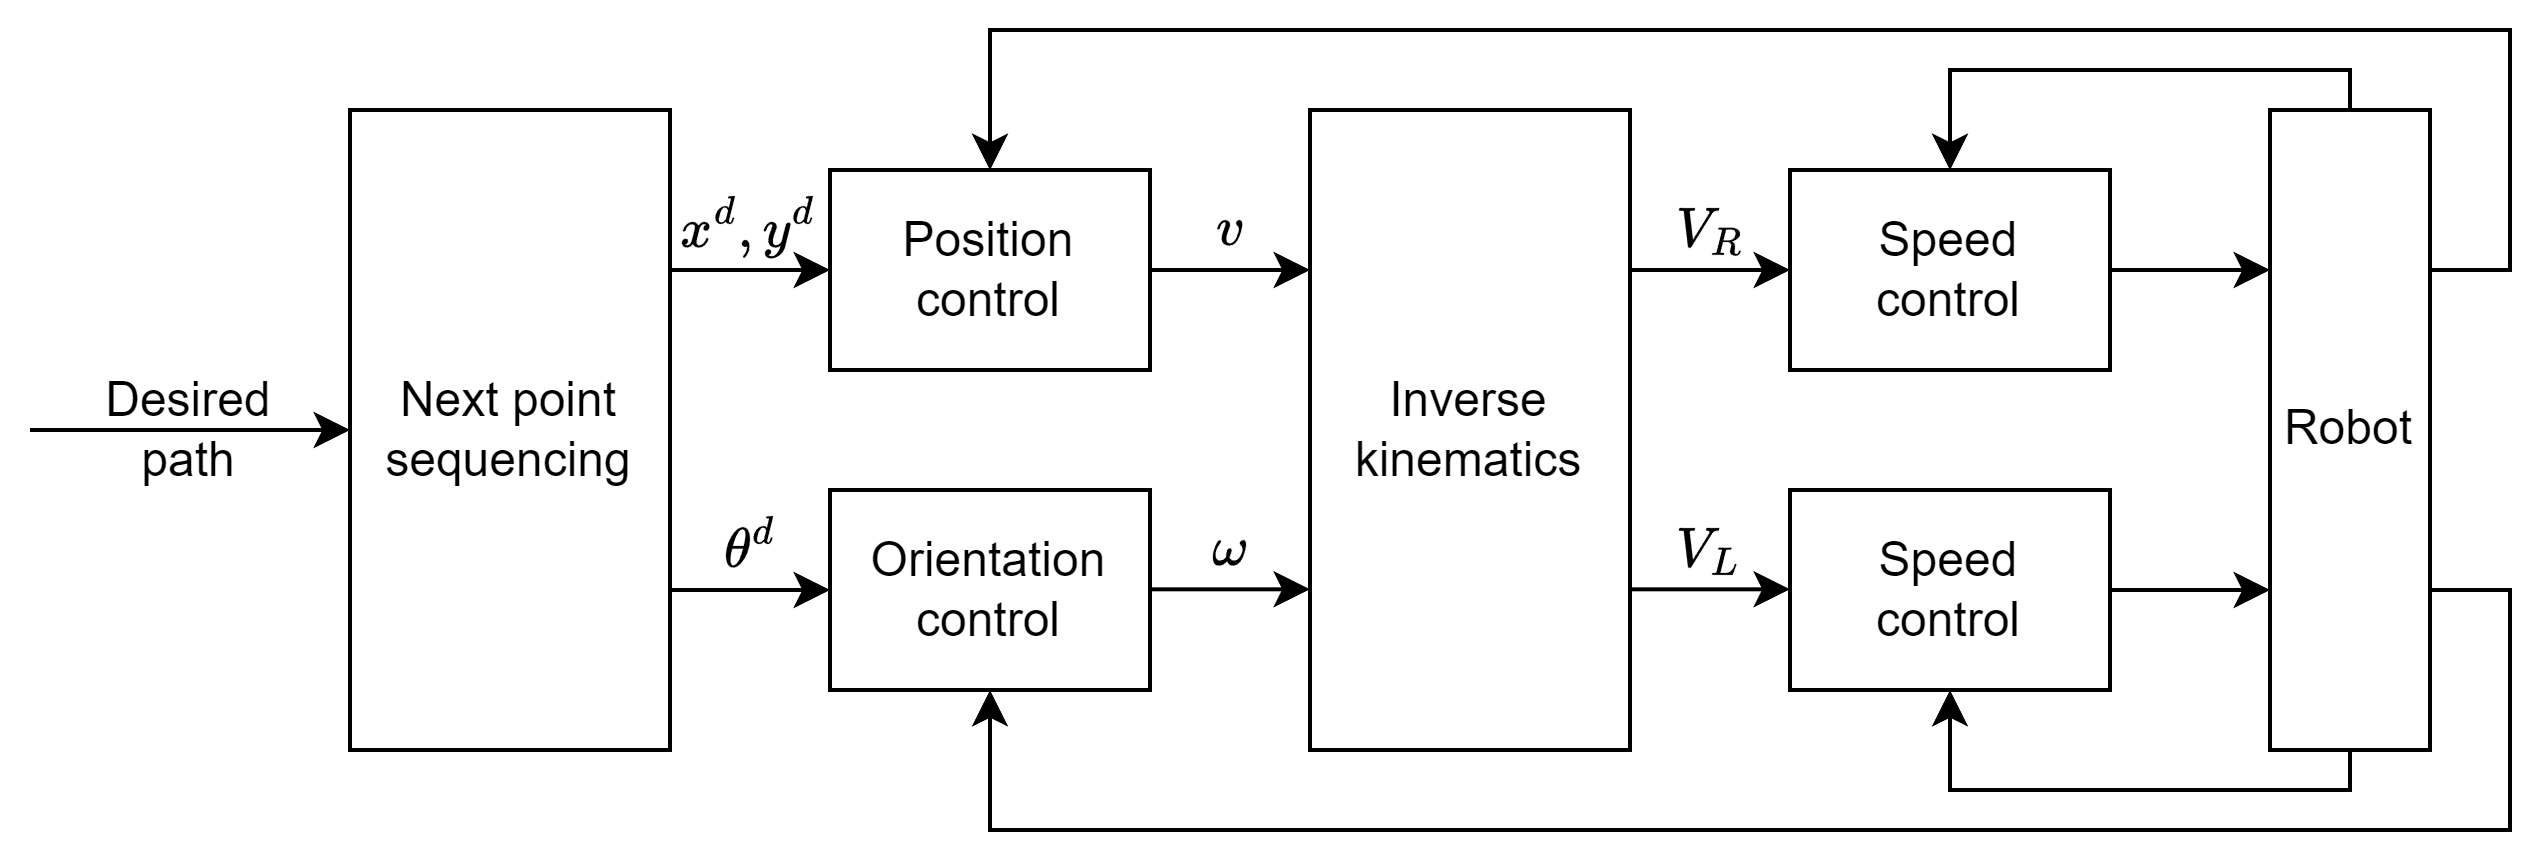
\includegraphics[width=0.75\linewidth]{images/fed.png}
    \caption{Feedback control for a differential drive robot}
\end{figure}
The primary challenge within this framework arises from the occurrence of temporary obstacles that alter the planned path.